
The optimal baseline methods described above highlight the problem's complexity. Both methods suffer from the large number of motion-planning queries they have to perform to compute the cost measures on the corresponding search structures. For this purpose it needs to be seen whether it is possible to decompose the problem into solvable sub-problems. 
%%%%%%%%%%%%%%%%%%%%%%%%%%%%%%%%%%%%%%%%%%%%%%%%%%%%%%%%%%%%%%
%%%%%%%%%%%%%%%%%%%%%%%%%%%%%%%%%%%%%%%%%%%%%%%%%%%%%%%%%%%%%%
%%%%%%%%%%%%%%%%%%%%%%%%%%%%%%%%%%%%%%%%%%%%%%%%%%%%%%%%%%%%%%
%%%%%%%%%%%%%%%%%%%%%%%%%%%%%%%%%%%%%%%%%%%%%%%%%%%%%%%%%%%%%%

\noindent\textbf{Importance of Transfers}: In order to draw some insight, consider again the tabletop setup with a general cost measure of $c_t$ per unit distance.
Lemma~\ref{l:k-arm-lower-bound} suggests that under certain conditions, there 
may not be a meaningful bound on the performance ratio between a $k$-arm 
solution and a single-arm solution. This motivates the examination of another
often used setting---randomly chosen non-overlapping 
start and goal locations for $n$ objects (within a unit square). In order to derive a 
meaningful bound on the benefit of using a $2$-arm solution 
to a single-arm solution, we first derive a conservative cost of a single-arm solution. 
A single-arm optimal cost has three main parts: 1) the portion of the transfer cost involving the pickup and 
drop-off of the $n$ objects with a cost of $C_{pd} = nc_{pd}$, 2) the remaining transfer cost from 
start to goal for all objects $C_{sg}$, and 3) the transit cost 
going from the goals to starts $C_{gs}$. The single arm cost is  
\vspace{-0.1in}
\begin{equation}
\label{eq:single-cost-exp}
C_{\rm single} = nc_{pd} + C_{sg} + C_{gs}.
\vspace{-0.1in}
\end{equation}
To estimate Eq.~\ref{eq:single-cost-exp}, first note that the randomized setup 
will allow us to obtain the expected $C_{sg}$\cite{santalo2004integral} as
$\frac{2 + \sqrt{2} + 5\ln(1+\sqrt{2})}{15}nc_t \approx 0.52nc_t$.
Approximate $C_{gs}$ by simply computing an optimal assignment of the 
goals to the starts of the objects excluding the matching of the same start 
and goal. Denoting the distance cost of this matching as $C_{gs}^M$, clearly
$C_{gs} > C_{gs}^M$ because the paths produced by the matching may form 
multiple closed loops instead of the desired single loop that connects all 
starts and goals. However, the number of loops produced by the matching 
procedure is on the order of $\ln n$ and therefore, $C_{gs} < C_{gs}^M + 
c_t\ln n$, by~\cite{TrePavFra13}. By \cite{AjtKomTus84}, 
$C_{gs}^M = \Theta(\sqrt{n\ln n})$. Putting these together, we have,

{\centerline
{
$\Theta(c_t\sqrt{n\ln n}) = C_{gs}^M < C_{gs} < C_{gs}^M + c_t\ln n 
= \Theta(c_t\sqrt{n\ln n}) + c_t\ln n$
}
}

\noindent which implies that $C_{gs} \approx C_{gs}^M$ because for large $n$, $\ln n
\ll \sqrt{n\ln n}$. It is estimated in \cite{yu2015target} that $C_{gs}^M 
\approx 0.44\sqrt{n\ln n}c_t$ for large $n$. Therefore, 

% \noindent Noting that the $0.44\sqrt{n\ln n}c_t$ term may also be ignored for large $n$,
% we have 
\vspace{-0.1in}
\begin{equation}\label{eq:single-cost-simple}
C_{\rm single} \approx nc_{pd} + (0.52n + 0.44\sqrt{n\ln n})c_t \approx (c_{pd} + 0.52c_t)n
% \vspace{-0.1in}
\end{equation}
noting that the $0.44\sqrt{n\ln n}c_t$ term may also be ignored for large $n$. The cost of dual arm solutions will be analyzed in Section \ref{sec:cost_bounds}.
{
\lemma For large $n$, the transfers dominate the cost of the solution.
\label{lem:transferdomination}
}
%%%%%%%%%%%%%%%%%%%%%%%%%%%%%%%%%%%%%%%%%%%%%%%%%%%%%%%%%%%%%%
%%%%%%%%%%%%%%%%%%%%%%%%%%%%%%%%%%%%%%%%%%%%%%%%%%%%%%%%%%%%%%
%%%%%%%%%%%%%%%%%%%%%%%%%%%%%%%%%%%%%%%%%%%%%%%%%%%%%%%%%%%%%%
%%%%%%%%%%%%%%%%%%%%%%%%%%%%%%%%%%%%%%%%%%%%%%%%%%%%%%%%%%%%%%

We formulate a strategy to reflect this importance of transfers.
The proposed approach gives up on the optimality of the complete problem, instead focusing on a high-quality solution, which:
\begin{myitem}
\item[$-$] first optimizes transfers and selects an assignment of object pairs to arms, 
\item[$-$] and then considers move costs and optimizes the schedule of assignments.
\end{myitem} 
This ends up scaling better by effectively reducing the size of the search space and performing fewer motion planning queries. It does so by optimizing a related cost objective and taking advantage of efficient polynomial-time algorithms. 

\begin{minipage}{0.48\textwidth}
  \begin{align}
  \label{eq:transfergraph}
  \begin{split}
  \graph(\nodes, \edges)\\
  \nodes = \{ \node=\object, \forall \object \in \objectset \}\\
  \edges = \{ \edge(u, v): \coma = (u,v), \forall u,v\in\nodes \}\\
  \cost(\edge(u,v)) = \cost(T(\coma=(u,v)))
  \end{split}
  \end{align}
\end{minipage}
\begin{minipage}{0.48\textwidth}
  \begin{align}
  \label{eq:transitgraph}
  \begin{split}
  \tspgraph(\tspnodes, \tspedges)\\
  \tspnodes = \{ \node=\coma, \forall \coma \in \scomaset^* \} \cup \{\coma_S\} \\
  \tspedges = \{ \edge(u, v): \coma_{u\rightarrow v}, \forall u,v\in\tspnodes \}\\
  \cost(\edge(u,v)) = \cost(M(\coma_{u\rightarrow v}))
  \end{split}
  \end{align}
\end{minipage}
\vspace{0.05in}

% \begin{align*}
% \ainit \rightarrow \atarget \\
% \scomaset^*\ \mathtt{on}\ \graph \\
% \scoma^+ : \tour \ \mathtt{on}\ \tspgraph
% \end{align*}

\begin{wrapfigure}{r}{2.5in}\vspace{-0.5in}
% \begin{figure}[H]
	\begin{center}
% 		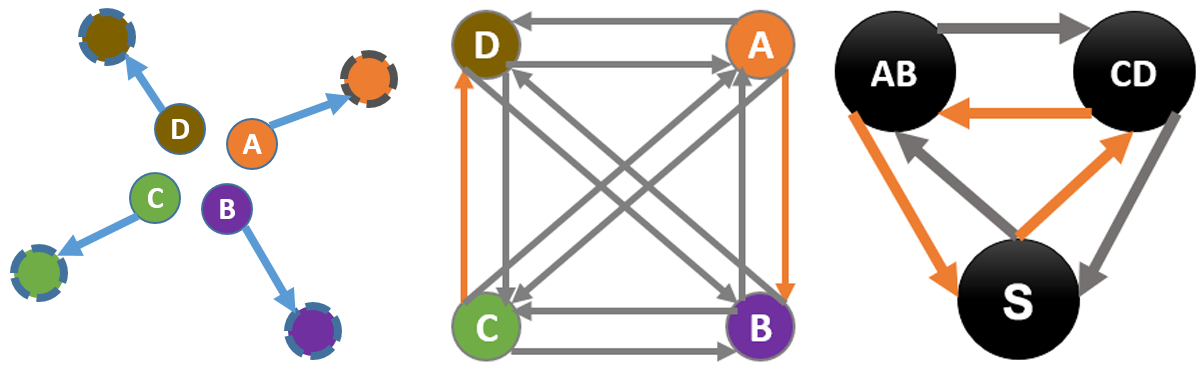
\includegraphics[width=2.5in]{figures/mapp}
		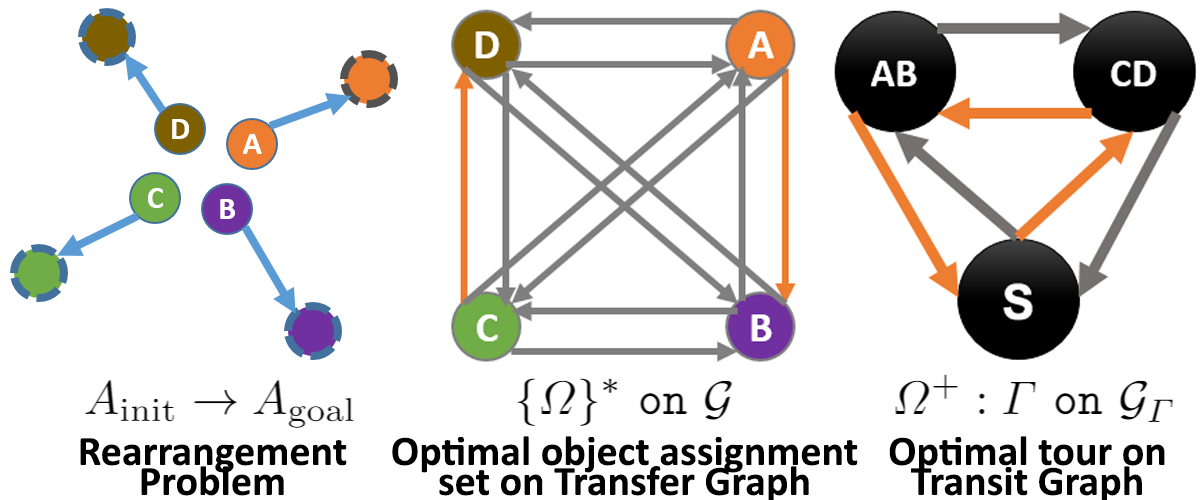
\includegraphics[width=2.5in]{figures/mapp_labels}
	\end{center}\vspace{-0.2in}
	\caption{(left) A dual-arm rearrangement problem. (middle) The same problem as minimum weight edge matching on a fully connected directed graph of \textit{transfers}. (right) The ordering of the object-arm assignments from an optimal tour over a \textit{transit} graph.}\vspace{-0.2in}
	\label{fig:edge_matching}
% \end{figure}
\vspace{-0.1in}
\end{wrapfigure}

\noindent\textbf{Foundations:} Consider a complete weighted directed graph $\graph(\nodes,\edges)$ (Eq.~\ref{eq:transfergraph}), where $\node \in \nodes$ corresponds to a single object $ \object $. Each directed edge, $\edge=(\object_i,\object_j) \in \edges$ is an ordered pair of objects $ \object_i $ and $\object_j $, where the order determines the assignment of an object to an arm $ \arm^1 $ or $ \arm^2 $. The cost of an edge $ \cost(\edge) $ is the coordinated motion planning cost of performing the transfer corresponding to $ \coma = (\object_i,\object_j) $. For instance, as shown in Fig \ref{fig:edge_matching}(middle), $\edge(A,B)$ corresponds to $ \arm^1 $ transferring `A', while $ \arm^2 $ transfers `B', and the $\cost( \edge(A,B) ) = \cost(T(\coma=(A,B))$ is the cost of such a concurrent motion. Note that these costs refer to only the transfer costs i.e., starting from the arms picking up the objects $ A $ and $ B $ at the initial poses(as shown in Fig \ref{fig:edge_matching}(left)), and moving them to their target poses. It should also be noted that since the arms are different, in general, $\cost( \edge(A,B) )$ is not necessarily equal to $\cost( \edge(B,A) )$.



Following the observation made in Eq.~\ref{eq:cost_function}, the cost of the transfers can be reasoned about independent of their order. 
Define $\scomaset$ as the unordered set of $\coma\in\scoma$, then unordered transfer cost component corresponds to $\sum_{\coma\in\scomaset}\cost(T(\coma))$.
% We defined $ \scoma $ to be an ordered sequence of object-to-arm assignments. Let $ \scoma $ be a candidate solution to the synchronized dual-arm rearrangement problem. $ \scoma $ is an ordered sequence of $ \coma $, and $ \scomaset $ denote the unordered set of all $ \coma $ that comprise $ \scoma $. 
Since $ \graph $ is a complete graph where every edge corresponds to every possible valid $ \coma $, $ \scomaset $ must also be a part of $ \graph $. 
From the construction of the graph $ \graph $, $ \scomaset \subset \edges$. By definition, a candidate solution of a monotone dual-arm rearrangement problem must transfer every object exactly once. In terms of the graph, this means that in the subset of edges $ \scomaset $ every vertex appears in only one edge. We arrive at the following crucial observation.



{\lemma [Perfect Matching]
Every candidate solution to a monotone dual-arm rearrangement problem comprises of a set of unordered object-to-arm assignments $ \scomaset $ that is also a perfect matching solution on $ \graph $.
}

As per the decomposition of the costs in Eq. \ref{eq:cost_function}, it follows that the $ \cost(\scomaset) $ corresponds to the cost of the transfers in the solution. Given the reduction to edge-matching, the solution to the minimum-weight perfect edge matching problem on such a graph would correspond to a $ \scomaset $ that optimizes the cost of \textit{transfers} of all the objects.

{\lemma [Optimal Matching]
The set of object-to-arm assignments $ \scomaset^* $ that minimizes the cost of object transfers is a solution to the minimum-weight perfect matching problem on $ \graph $.
}
% $$
% \scomaset^* = \underset{ \scomaset \in \mathtt{EM(\graph)}  }{ \mathtt{argmin} } \ \cost(\scomaset)
% $$

Once such an optimal assignment $ \scomaset^* $ is obtained, the missing part of the complete solution is the set of transits between the object transfers and their ordering. Construct another directed graph $ \tspgraph $ (Eqs. \ref{eq:transitgraph}), where the vertices comprise of the $ \coma \in \scomaset^*$. An edge $ e(\coma_{u\rightarrow v}) $ between any two vertices corresponds to the coordinated \textit{transit} motion between them. For instance, as in Fig \ref{fig:edge_matching}(right) for an edge between $ \coma(A,B) $ and $ \coma(C,D) $, $ \arm^1 $ moves from the target pose of object `A' to the starting pose of object `C', and similarly $ \arm^2 $ moves from the target of `B' to the start of `D'. An additional vertex corresponding to the starting(and ending) configuration of the two arms ($ \startq $) is added to the graph. The graph is fully connected again to represent all possible transits or moves.  


A complete candidate solution to the problem now requires the sequence of~$ \coma $. By definition of the edges, the complete solution begins at~$ \startq $ and also ends there. This is a complete tour over~$ \tspgraph $, that visits all the vertices i.e., an ordered sequence of vertices $\tour = ( {\startq}, \scoma_\tour, {\startq}  )$.

{
\lemma [Tour]
Any complete tour $ \tour $ over the graph $ \tspgraph $, corresponds to a sequence of object-to-arm assignments $ \scoma_\tour $ and is a candidate solution to the synchronous dual-arm rearrangement problem.
}

% In the problem setup it was assumed that $ \trajset(\scoma) $ contained the start and end transits to $ \startq $. Additionally, the entire trajectory contained both transfers and transits. Since we have considered all the transfers in $ \cost(\scomaset^*) $, what remains is the transits. Then 
% The cost of the tour $ \tour $ can be written as $\cost(\tour) = \sum_{e(u,v)\in\tour}\cost({M}( \coma_{u\rightarrow v} ))$.


Let $ \mathbb{P}^{\scomaset} $ represent the set of all possible ordering of the elements in $ \scomaset $. This means, any candidate tour corresponds to a $ \scoma_\tour\in\mathbb{P}^{\scomaset} $. An optimal tour on $ \tspgraph $ minimizes the transit costs over the all possible candidate solutions in  $ \mathbb{P}^{\scomaset^*} $.
\vspace{-0.1in}
\begin{equation}
\scoma^+ = \underset{ \scoma \in  \mathbb{P}^{\scomaset^*}   }{ \mathtt{argmin} } \ \sum_{e(u,v)\in\tour}\cost({M}( \coma_{u\rightarrow v} ))  )
\vspace{-0.05in}
\end{equation}

This differs from the true optimal $ \scoma^* $, since the second step of finding the optimal transit tour only operates over all possible solutions that include the optimally matched transfers obtained in the first step.
The insight here is that, even though $ \scoma^+ $ reports a solution to a hierarchical optimization objective, the algorithm operates over a much smaller search space, and operates over sub-problems which are more efficient to solve than the baselines.\\

\noindent\textbf{Algorithm}: This section describes the algorithm {\tt {Tour\_Over\_Matching}} (\algo) outlined in the previous section. The steps correspond to Algo \ref{algo:tom}. 
% The algorithm takes as input the set of objects $ \objectset $ and the start(and end) configuration $ \startq $ of the arms.

\noindent $ \mathtt{transfer\_graph} $: This function constructs a directed graph $ \graph $ defined by Eqs.~\ref{eq:transfergraph}. This step creates a graph with $ n $ vertices and $ \permu[n]{2} $ edges.

\begin{wrapfigure}{r}{0.6\textwidth}\vspace{-0.3in}
  \begin{minipage}{0.6\textwidth}
  \vspace{0pt} 
    \begin{algorithm}[H]
    \caption{{\tt \algo}$ (\objectset, \startq, \ainit, \atarget) $}
    \label{algo:tom}
    $ \graph \leftarrow \mathtt{transfer\_graph}(\objectset, \ainit, \atarget) $\;
    $ \scomaset^* \leftarrow \mathtt{optimal\_matching}(\graph) $\;
    $ \tspgraph \leftarrow \mathtt{transit\_graph}(\scomaset^*, \startq) $\;
    $ \scoma^+\leftarrow\mathtt{optimal\_tour}(\tspgraph) $\;
    $ \mathbf{\mathtt{return}}\ \trajset(\scoma^+)$\;
    \end{algorithm}
  \end{minipage}
  \vspace{-0.3in}
\end{wrapfigure}

\noindent $ \mathtt{optimal\_matching} $: This function takes the graph $ \graph $ constructed as an argument and returns the unordered set of edges, corresponding to the set of optimal transfers over $ \graph $. 
\commentdel{The first step is to convert the directed graph $ \graph $ into an equivalent undirected graph $ \graph_U $. Since $ \graph $ is complete, every pair of vertices has two directed edges between them. $\graph_U$ only preserves the minimally weighted connection for every vertex pair. Optimal matching is solved using an Edmond's Blossom Algorithm~\cite{edmonds1965maximum,galil1986ev} implementation~\cite{dezsHo2011lemon}. 
% Since the algorithm performs maximum matching by default, our desired minimally weighted matching can be obtained by subtracting the edge weights from some arbitrarily large number.
}
\commentadd{Optimal matching over an undirected graph can be solved using Edmond's Blossom Algorithm~\cite{edmonds1965maximum,galil1986ev,dezsHo2011lemon}. The directed graph $ \graph $ is converted into an equivalent undirected graph $ \graph_U $. Since $ \graph $ is complete, every pair of vertices shares two directed edges. $\graph_U$ only preserves the minimally weighted connection for every vertex pair. The result of matching}
% The result 
is a subset of edges on $ \graph_U $ which correspond to a set of directed edges on $ \graph $ i.e., $ \scomaset^* $. The runtime complexity of the step is $ O(|\edges||\nodes|\log|\nodes|) = O(\permu[n]{2}n\log n ) = O(n^3\log n)$.

\noindent $ \mathtt{transit\_graph} $: This function constructs the directed transit graph $ \tspgraph $ as per the set of Eqs.~\ref{eq:transitgraph}. This constructs $ \frac{n}{2} + 1 $ vertices and $ \permu[(\frac{n}{2} + 1)]{2} $ edges.

\noindent $\mathtt{optimal\_tour}  $: Standard TSP solvers like Gurobi~\cite{gurobi} can be used to find the  
% It should be noted that a lot of efficient solvers exist for such problems, that provide various degrees of approximation. 
optimal tour over $ \tspgraph $ corresponding to $ \scoma^+ $.

The costs are deduced from coordinated motion plans over edges. The total number of such calls compared to the count from the baseline in Equ. \ref{eq:mpcount}, shows a saving in the order of $ O(n^2)$ queries ($\textrm{\# of Transfers} + \textrm{\# of Moves}$). 
% \kiril{Consider completing the calculation.}
\vspace{-0.1in}
$$
\frac{\textrm{Baseline}\ \#}{{\algo}\ \#} = 
\frac{  {\permu[n]{2}} +   \Big{(}{{\permu[n]{2}}\times\permu[n-2]{2}}\Big{)} + \Big{(}2\times{\permu[n]{2}}\Big{)}   }
{\permu[n]{2} + \permu[(\frac{n}{2} + 1)]{2}} =
\frac{4(n-1)((n-5)n+9)}{5n-2}
$$\vspace{-0.1in}

The evaluation performed here focuses on the maximum of distances (Eq.~\ref{eq:cost_function}) for a fair comparison with the other methods. The prioritization of optimization objective, however, is also amenable to other cost functions, where carrying objects is often more expensive than object-free motions. 